% https://tex.stackexchange.com/questions/264260/matrix-product-illustration?noredirect=1&lq=1
\documentclass{standalone}
\usepackage{tikz}
\usetikzlibrary{matrix,arrows.meta,positioning}

\definecolor{myyellow}{RGB}{240,217,1}
\definecolor{mygreen}{RGB}{143,188,103}
\definecolor{myred}{RGB}{234,38,40}
\definecolor{myblue}{RGB}{53,101,167}

\begin{document}

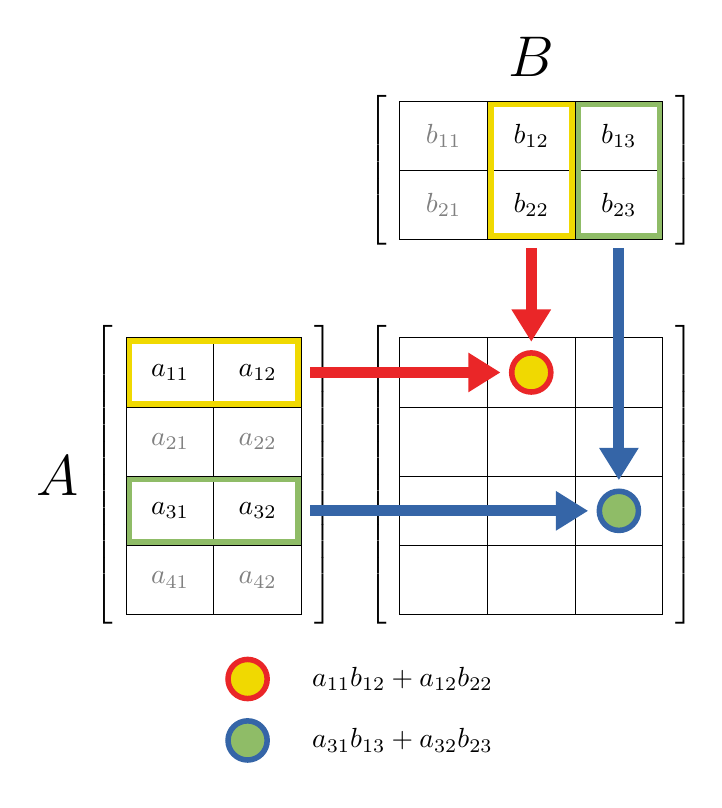
\begin{tikzpicture}[
mymatrix/.style={
  matrix of math nodes,
  outer sep=0pt,
  nodes={
    draw,
    text width=2.5em,
    align=center,
    minimum height=2.5em,
    text=gray
  },
  nodes in empty cells,
  column sep=-\pgflinewidth,
  row sep=-\pgflinewidth,
  left delimiter=[,
  right delimiter=],
  },
  mycircle/.style 2 args={
    draw=#1,
    circle,
    fill=#2,
    line width=2pt,
    inner sep=5pt
  },
  arr/.style={
  line width=4pt,
  -{Triangle[angle=60:1.5pt 3]},
  #1,
  shorten >= 3pt,
  shorten <= 3pt
  }
]
%the matrices
\matrix[mymatrix] (A)
{
|[text=black]|a_{11} & |[text=black]|a_{12} \\
a_{21} & a_{22} \\
|[text=black]|a_{31} & |[text=black]|a_{32} \\
a_{41} & a_{42} \\
};
\matrix[mymatrix,right=of A.north east,anchor=north west] (prod)
{
& & \\
& & \\
& & \\
& & \\
};
\matrix[mymatrix,above=of prod.north west,anchor=south west] (B)
{
b_{11} & |[text=black]|b_{12} & |[text=black]|b_{13} \\
b_{21} & |[text=black]|b_{22} & |[text=black]|b_{23} \\
};

%the labels for the matrices
\node[font=\huge,left=10pt of A] {$A$};
\node[font=\huge,above=2pt of B] {$B$};

%the frames in both matrices
\draw[myyellow,line width=2pt]
  ([shift={(1.2pt,-1.2pt)}]A-1-1.north west) 
  rectangle 
  ([shift={(-1.2pt,1.2pt)}]A-1-2.south east);
\draw[myyellow,line width=2pt]
  ([shift={(1.2pt,-1.2pt)}]B-1-2.north west) 
  rectangle 
  ([shift={(-1.2pt,1.2pt)}]B-2-2.south east);
\draw[mygreen,line width=2pt]
  ([shift={(1.2pt,-1.2pt)}]A-3-1.north west) 
  rectangle 
  ([shift={(-1.2pt,1.2pt)}]A-3-2.south east);
\draw[mygreen,line width=2pt]
  ([shift={(1.2pt,-1.2pt)}]B-1-3.north west) 
  rectangle 
  ([shift={(-1.2pt,1.2pt)}]B-2-3.south east);

%the filled circles in the product
\node[mycircle={myblue}{mygreen}]
  at (prod-3-3) (prod33) {};
\node[mycircle={myred}{myyellow}]
  at (prod-1-2) (prod12) {};

%the arrows
\draw[arr=myred]
  (A-1-2.east) -- (prod12); 
\draw[arr=myred]
  (B-2-2.south) -- (prod12); 
\draw[arr=myblue]
  (A-3-2.east) -- (prod33); 
\draw[arr=myblue]
  (B-2-3.south) -- (prod33); 

%the legend
\matrix[
  matrix of math nodes,
  nodes in empty cells,
  column sep=10pt,
  anchor=north,
  nodes={
    minimum height=2.2em,
    minimum width=2em,
    anchor=north west
  },
  below=5pt of current bounding box.south
  ] 
  (legend)
{
  & a_{11}b_{12} + a_{12}b_{22} \\
  & a_{31}b_{13} + a_{32}b_{23} \\
};
\node[mycircle={myblue}{mygreen}]
  at (legend-2-1) {};
\node[mycircle={myred}{myyellow}]
  at (legend-1-1) {};
\end{tikzpicture}

\end{document}